\documentclass[12pt, oneside]{article} 
\usepackage{amsmath, amsthm, amssymb, calrsfs, wasysym, verbatim, bbm, color, graphics, geometry, multirow, booktabs}
\usepackage{graphicx}
\usepackage{tikz}
\usepackage{amsmath}
\usepackage{graphicx}
\usepackage{amsmath, amssymb, amsthm}
\usepackage{setspace}
\usepackage{tikz}
\usetikzlibrary{trees, positioning}
\usepackage{pgfplots}
\renewcommand{\baselinestretch}{1.0}
\geometry{tmargin=.75in, bmargin=.75in, lmargin=.75in, rmargin = .75in}  

\newcommand{\R}{\mathbb{R}}
\newcommand{\C}{\mathbb{C}}
\newcommand{\Z}{\mathbb{Z}}
\newcommand{\N}{\mathbb{N}}
\newcommand{\Q}{\mathbb{Q}}
\newcommand{\Cdot}{\boldsymbol{\cdot}}


\title{SP25 8732: Homework 2}
\author{Danbo CHEN}
\date{\today}

\begin{document}

\maketitle
\vspace{.25in}

\section{Question 1}
\textbf{(a) Solution:}

\begin{center}
    
    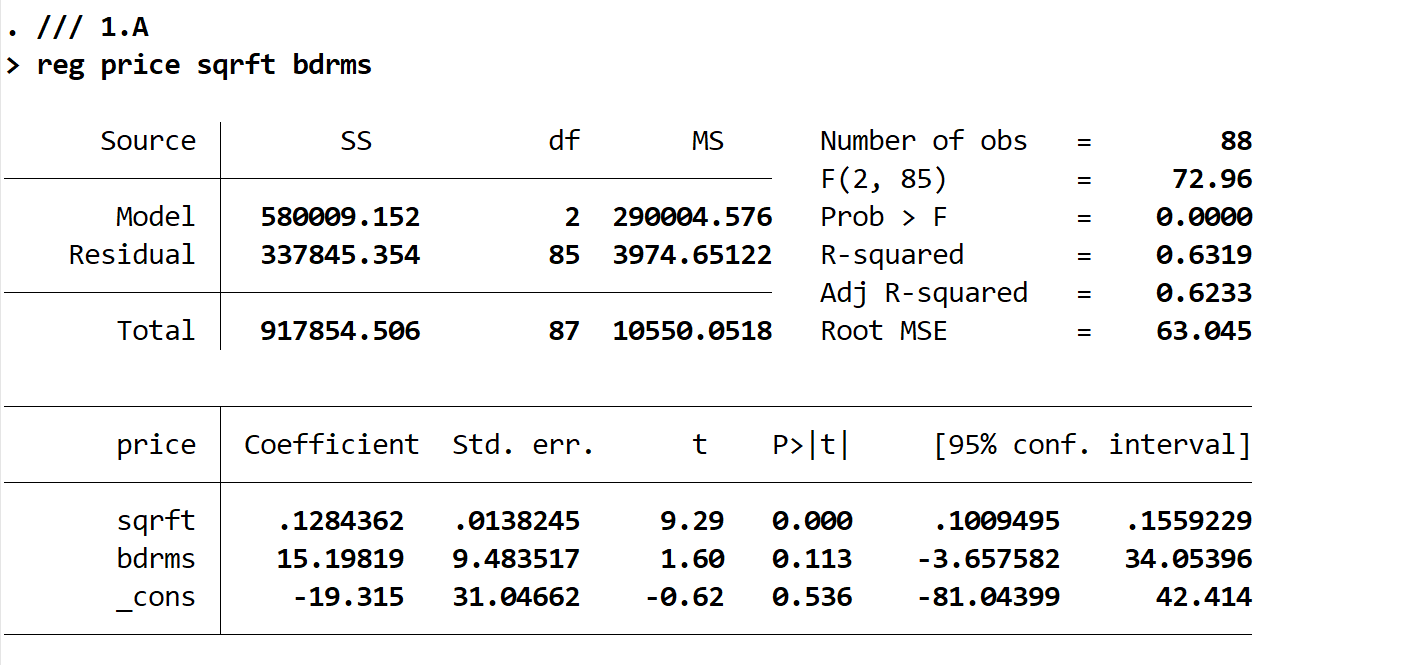
\includegraphics[width=0.8\textwidth]{Figure/P1.A.jpg}

    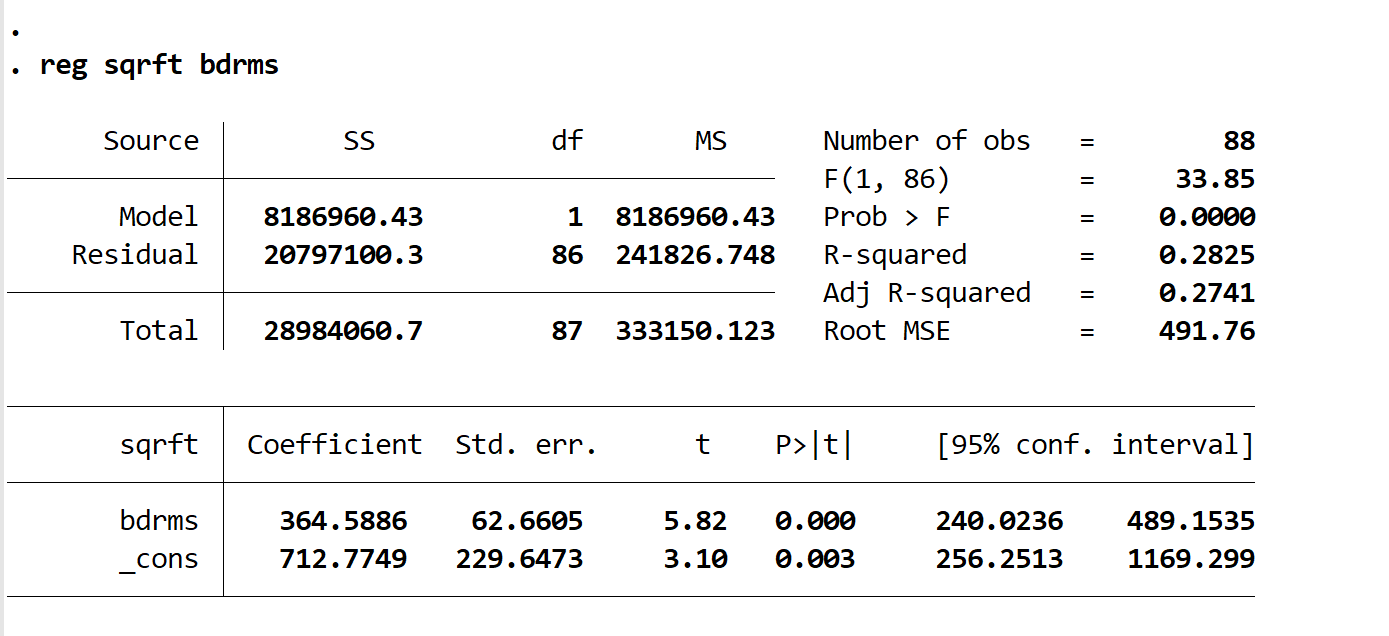
\includegraphics[width=0.8\textwidth]{Figure/P1.B.jpg}

    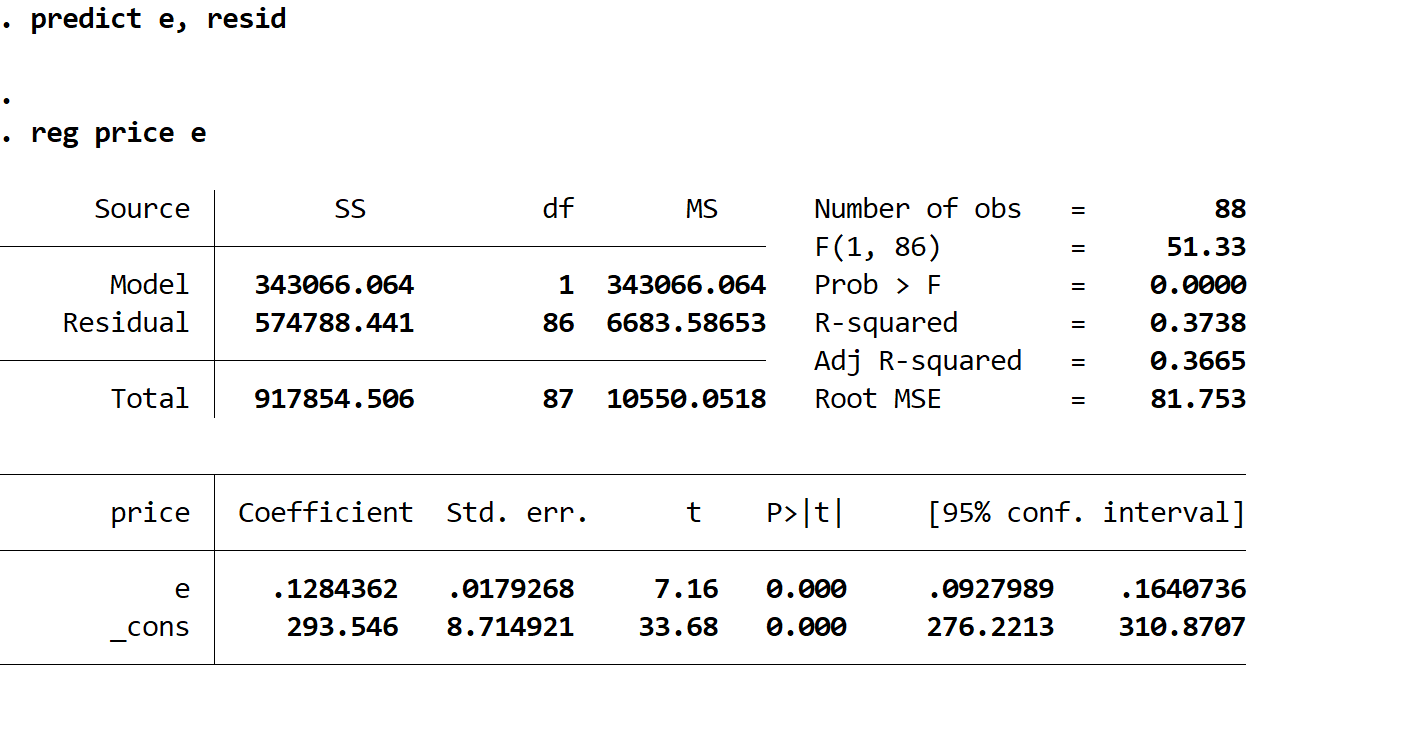
\includegraphics[width=0.8\textwidth]{Figure/P1.C.jpg}

\end{center}

The coefficients of the residual’s component $e_i$ are equal to the $\hat{\beta}_1$ estimated in the first regression. By definition, the coefficient $\hat{\beta}_1$ is the partial effect of $SQRFT_i$ on $PRICE_i$ holding everything else fixed. With this procedure, estimating the residuals of $SQRFT_i$ on $BDRMS_i$, we account for the variations in $SQRFT_i$ which does not depend on the variable $SQRFT_i$. In other words, we keep fixed the variation of $SQRFT_i$ due to change in $BDRMS_i$, and using the residuals we just see the partial effect of $SQRFT_i$ on prices.

\textbf{(b) Solution:}
\begin{center}
    
    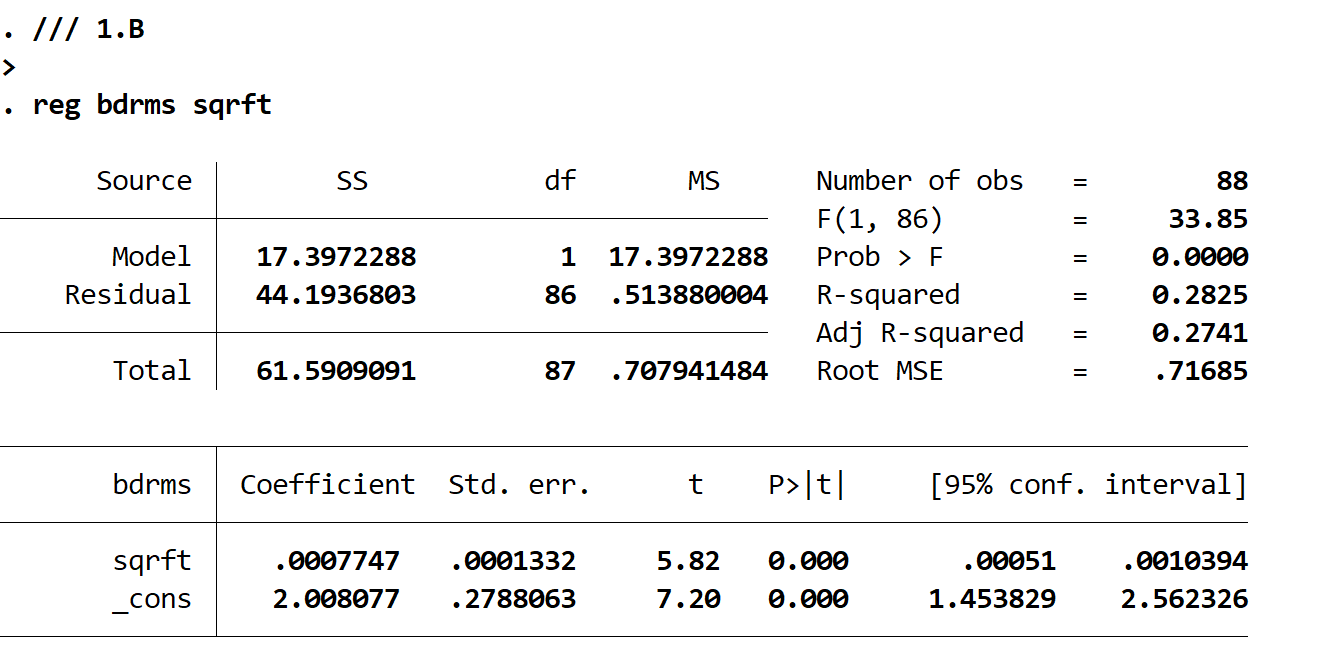
\includegraphics[width=0.8\textwidth]{Figure/P1.D.jpg}

    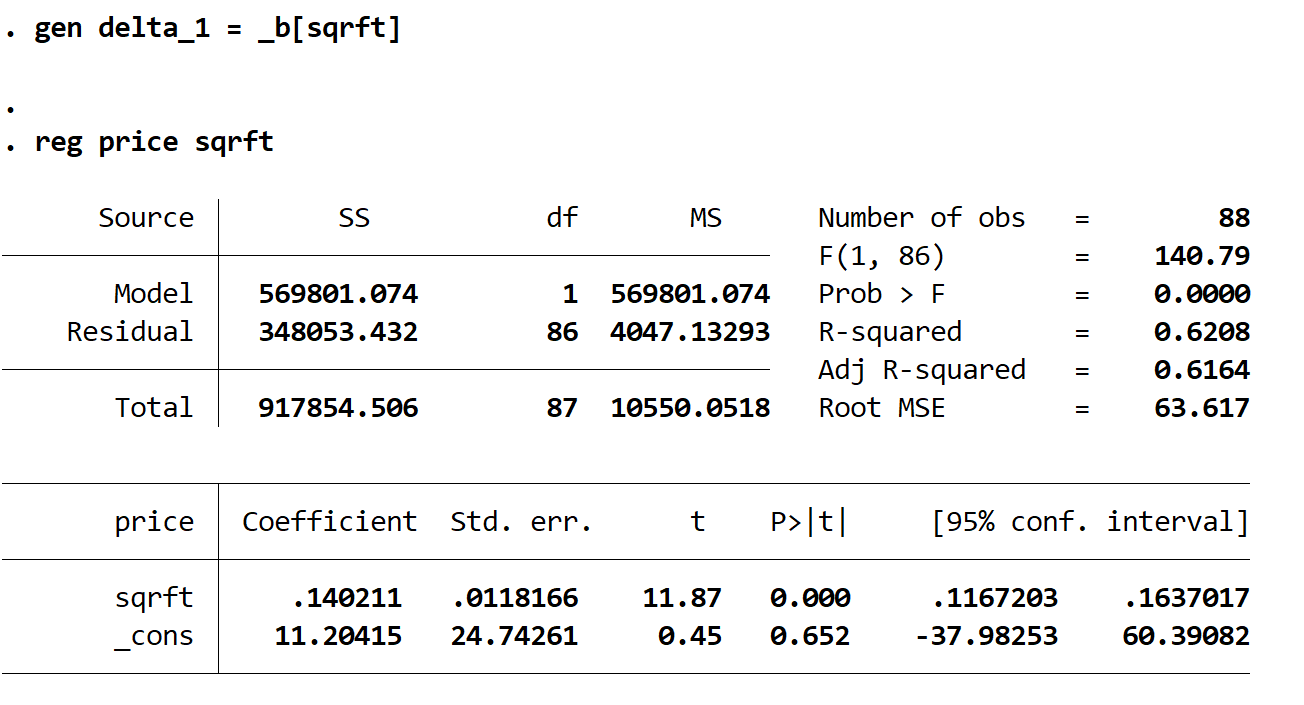
\includegraphics[width=0.8\textwidth]{Figure/P1.E.jpg}

    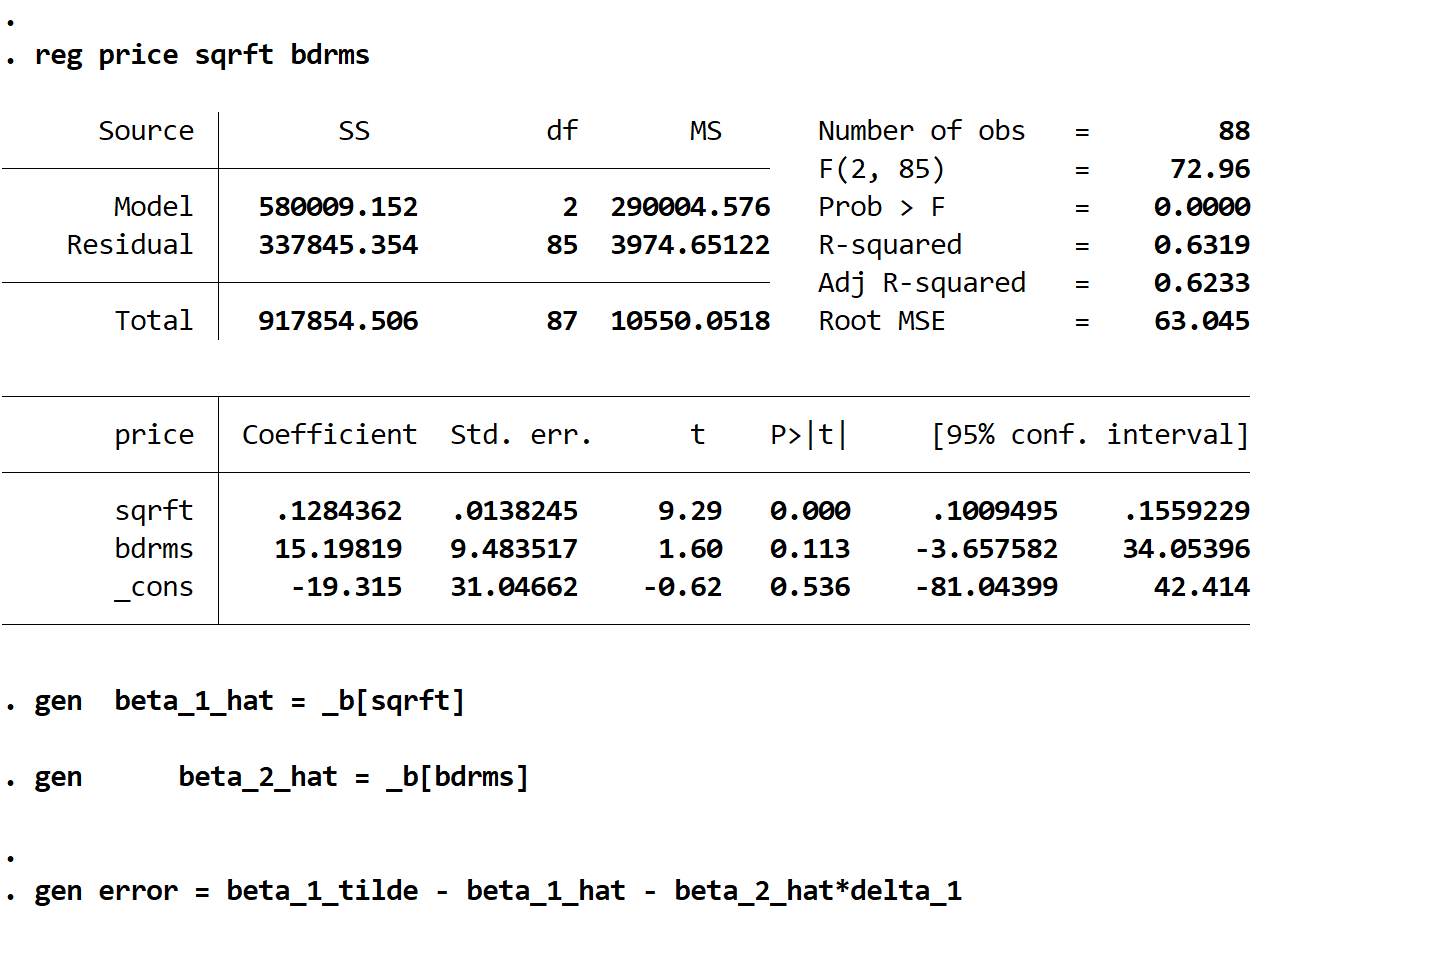
\includegraphics[width=0.8\textwidth]{Figure/P1.F.jpg}

\end{center}

Results are presented in Table 1.

\begin{table}[h]
    \centering
    \caption{Estimation results from above steps.}
    \begin{tabular}{ccccc}
        \toprule
        $\tilde{\delta}_1$ & $\tilde{\beta}_1$ & $\hat{\beta}_1$ & $\hat{\beta}_2$ & $\tilde{\beta}_1 - \hat{\beta}_1 - \hat{\beta}_2 \tilde{\delta}_1$ \\
        \midrule
        0.0007747 & 0.140211 & 0.1284362 & 15.19819 & -3.23e-09 \\
        \bottomrule
    \end{tabular}
\end{table}

We can verify that: 
\[
\tilde{\beta}_1 = \hat{\beta}_1 + \hat{\beta}_2 \tilde{\delta}_1
\]
To derive the expectation result, we take the conditional expectation on both sides and use the fact that the **OLS estimator** is conditionally unbiased:
\[
\mathbb{E}[\hat{\beta}_1] = \beta_1, \quad \mathbb{E}[\hat{\beta}_2] = \beta_2.
\]
Furthermore, **\(\tilde{\delta}_1\) is a function of the data matrix \(X\)**:
\[
\tilde{\delta}_1 = (X_1' X_1)^{-1} X_1' X_2.
\]
Thus:
\[
\mathbb{E}[\hat{\beta}_1 \mid X] = \mathbb{E}[\hat{\beta}_1 + \hat{\beta}_2 \tilde{\delta}_1 \mid X] = \beta_1 + \beta_2 \tilde{\delta}_1.
\]
We consider a regression model:
\[
Y_i = \beta_0 + \beta_1 X_{i1} + \beta_2 X_{i2} + \varepsilon_i,
\]
where **\(X_{i2}\) is omitted** from the regression. Define:
\[
X_i =
\begin{bmatrix} 1 \\ SQRFT_i \\ BDRMS_i \end{bmatrix}, \quad
Z_{i1} =
\begin{bmatrix} 1 \\ SQRFT_i \end{bmatrix}, \quad
Z_{i2} =
\begin{bmatrix} BDRMS_i \end{bmatrix}.
\]
Let:
\[
\gamma_1 = (\beta_0, \beta_1)', \quad \gamma_2 = (\beta_2).
\]

\[
\hat{\beta} = (Z_1'Z_1)^{-1} Z_1' Y.
\]
Substituting \( Y = Z\beta + \varepsilon \):
\[
\hat{\beta} = (Z_1'Z_1)^{-1} Z_1' (Z\beta + \varepsilon).
\]
Expanding:
\[
\hat{\beta} = \gamma_1 + P_{1.2} \gamma_2 + (Z_1'Z_1)^{-1} Z_1' \varepsilon.
\]
\textbf{Taking Expectation:}
\[
\mathbb{E}[\hat{\beta} \mid X] = \gamma_1 + P_{1.2} \gamma_2.
\]
Since \( Z_2 \) is a scalar, \( \gamma_2 = \beta_2 \), and:
\[
P_{1.2} = (\tilde{\delta}_0, \tilde{\delta}_1)'.
\]
Thus, we obtain:
\[
\mathbb{E}
\begin{bmatrix}
\hat{\beta}_0 \\ \hat{\beta}_1
\end{bmatrix}
\Bigg| X
=
\begin{bmatrix}
\beta_0 \\ \beta_1
\end{bmatrix}
+
\begin{bmatrix}
\tilde{\delta}_0 \\ \tilde{\delta}_1
\end{bmatrix}
\beta_2.
\]
The second row confirms the required result.

\section{Question 2}
\textbf{Solution:}

\begin{center}

    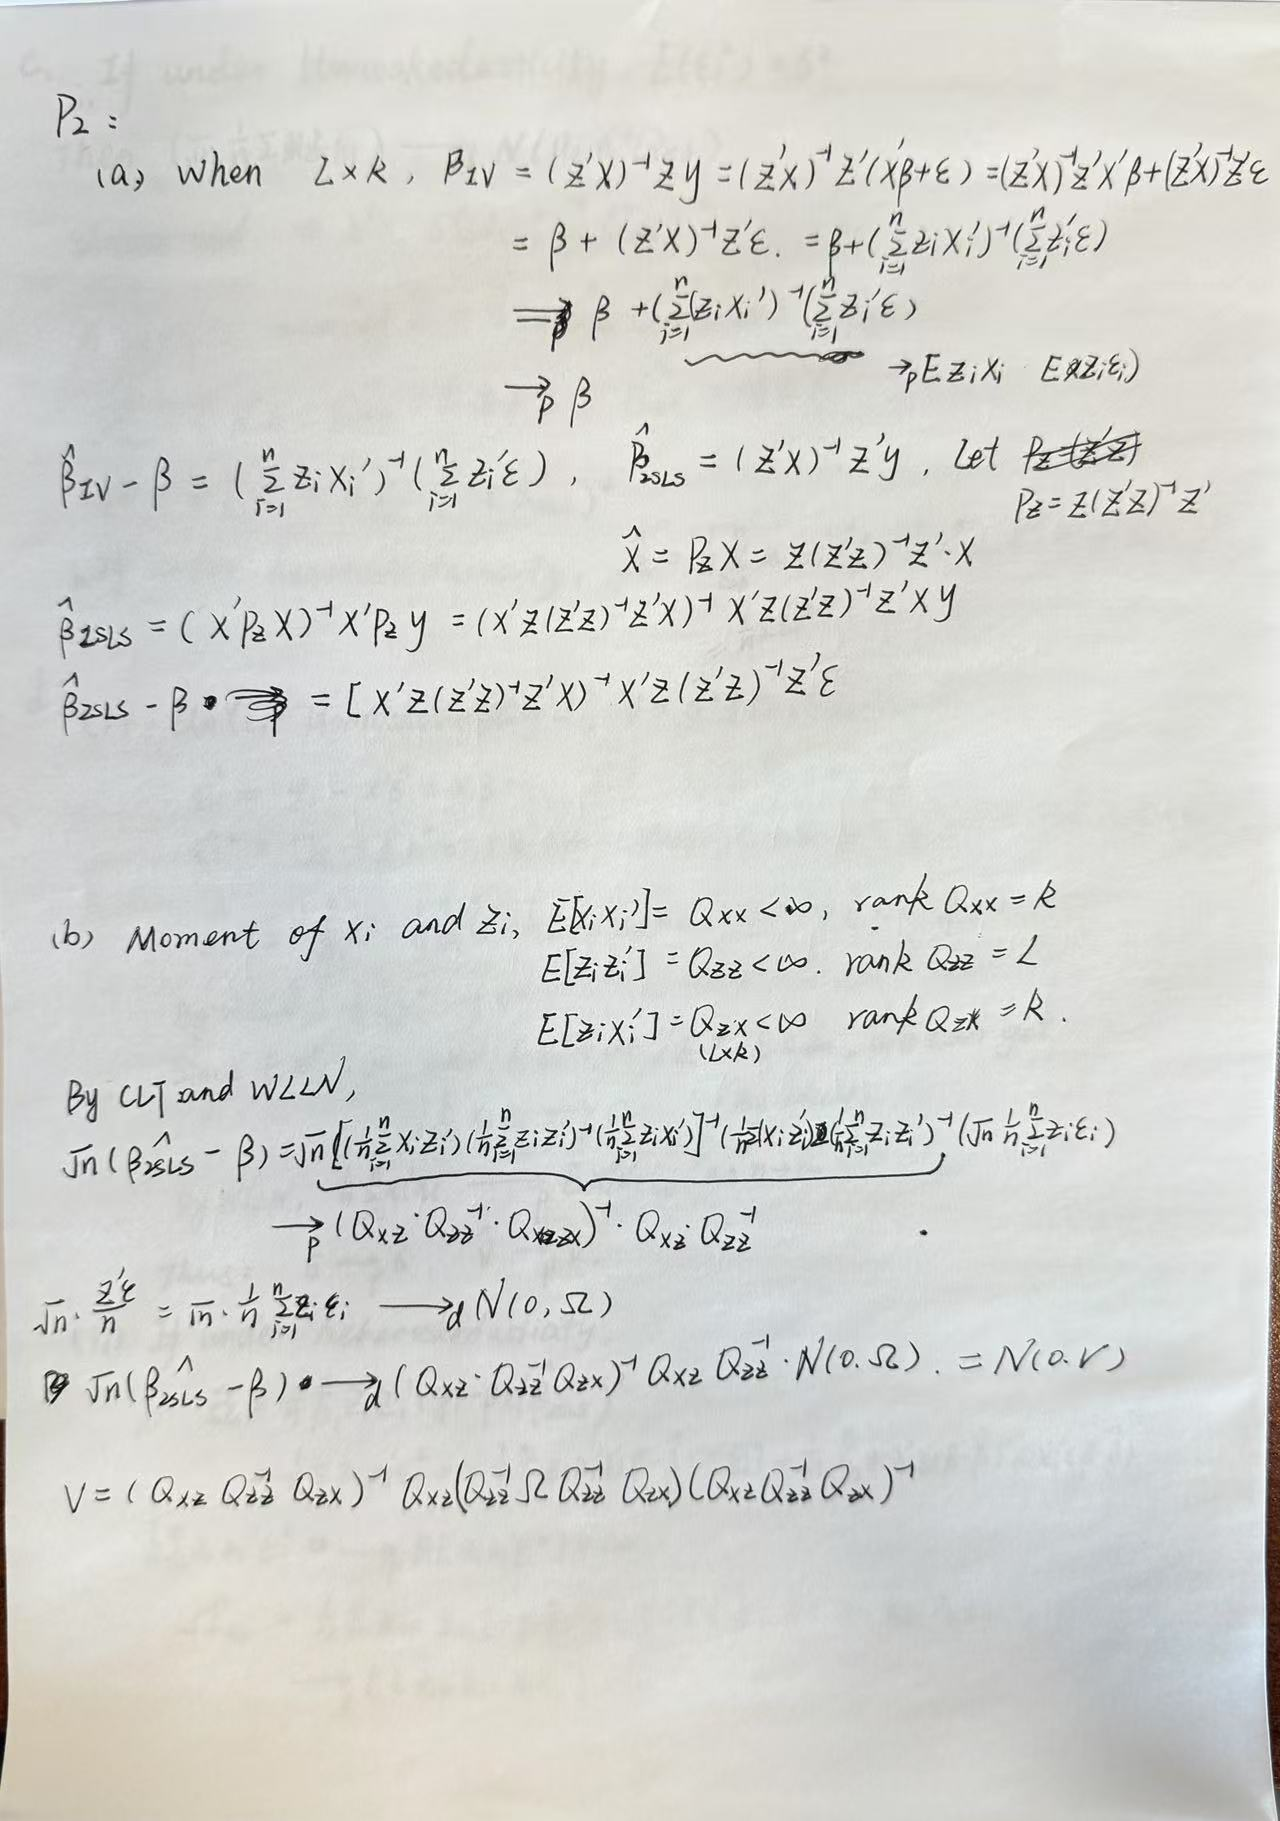
\includegraphics[width=0.8\textwidth]{Figure/P2.1.jpg}

    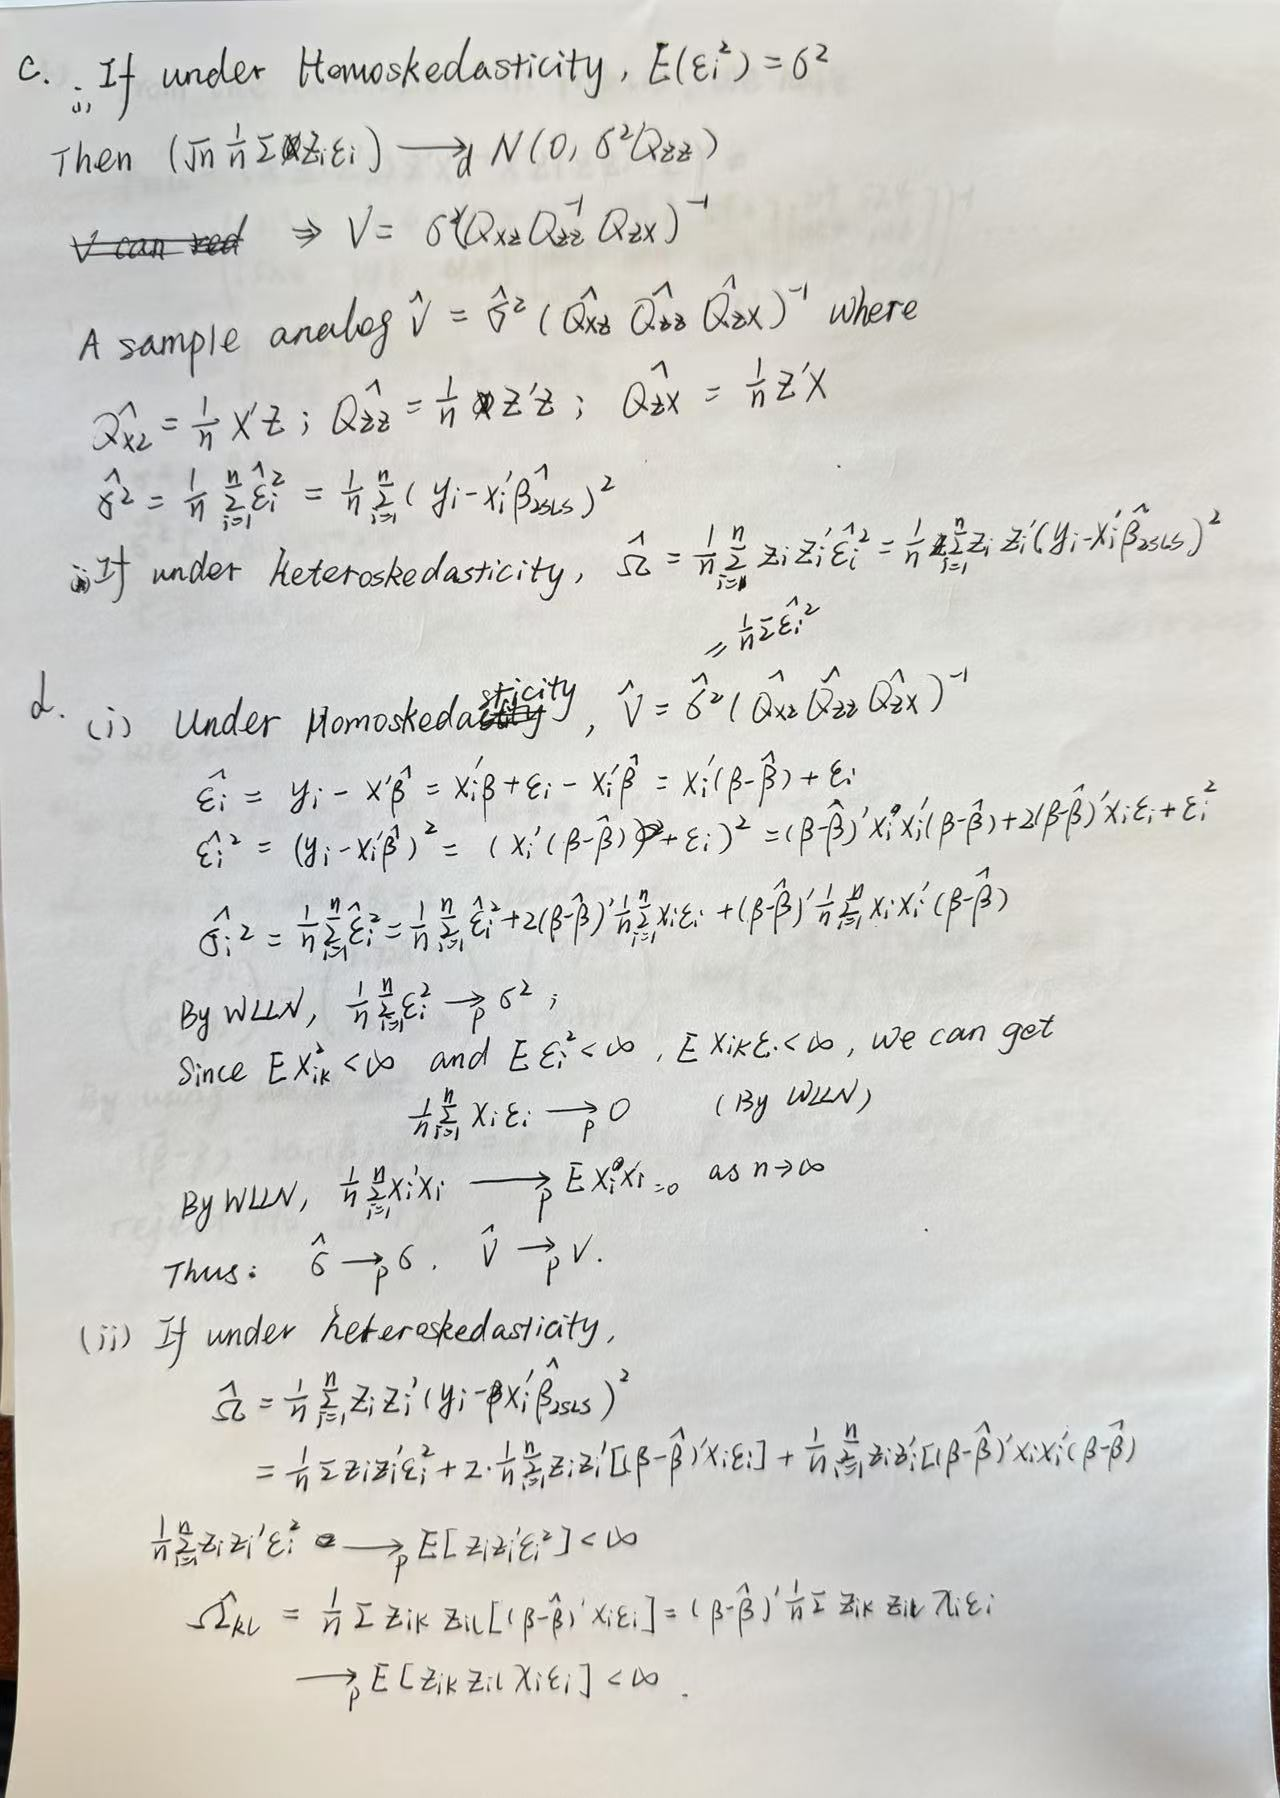
\includegraphics[width=0.8\textwidth]{Figure/P2.2.jpg}
\end{center}

\section{Question 3}
\textbf{Solution:}

\begin{center}

    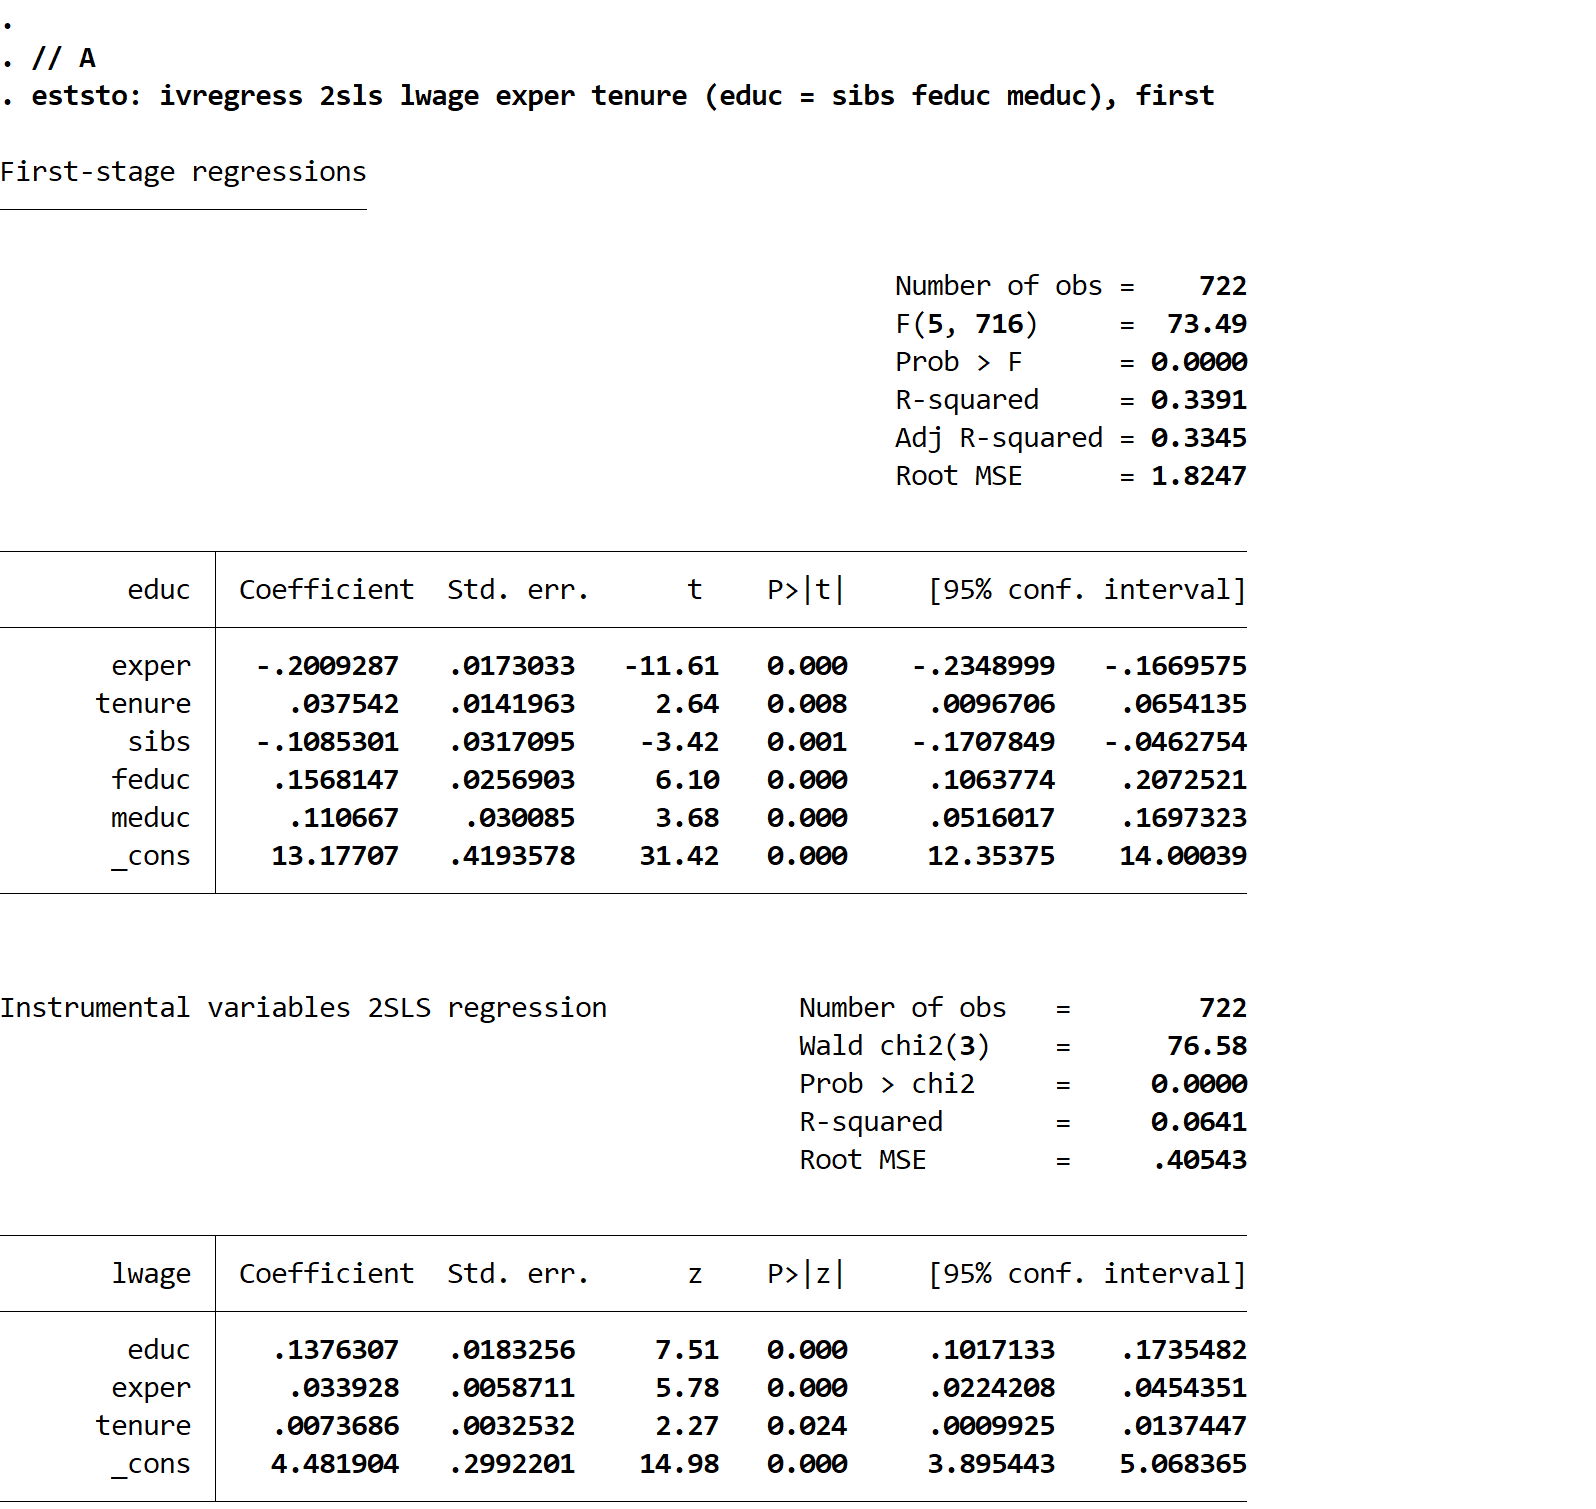
\includegraphics[width=0.8\textwidth]{Figure/P3.1.jpg}

    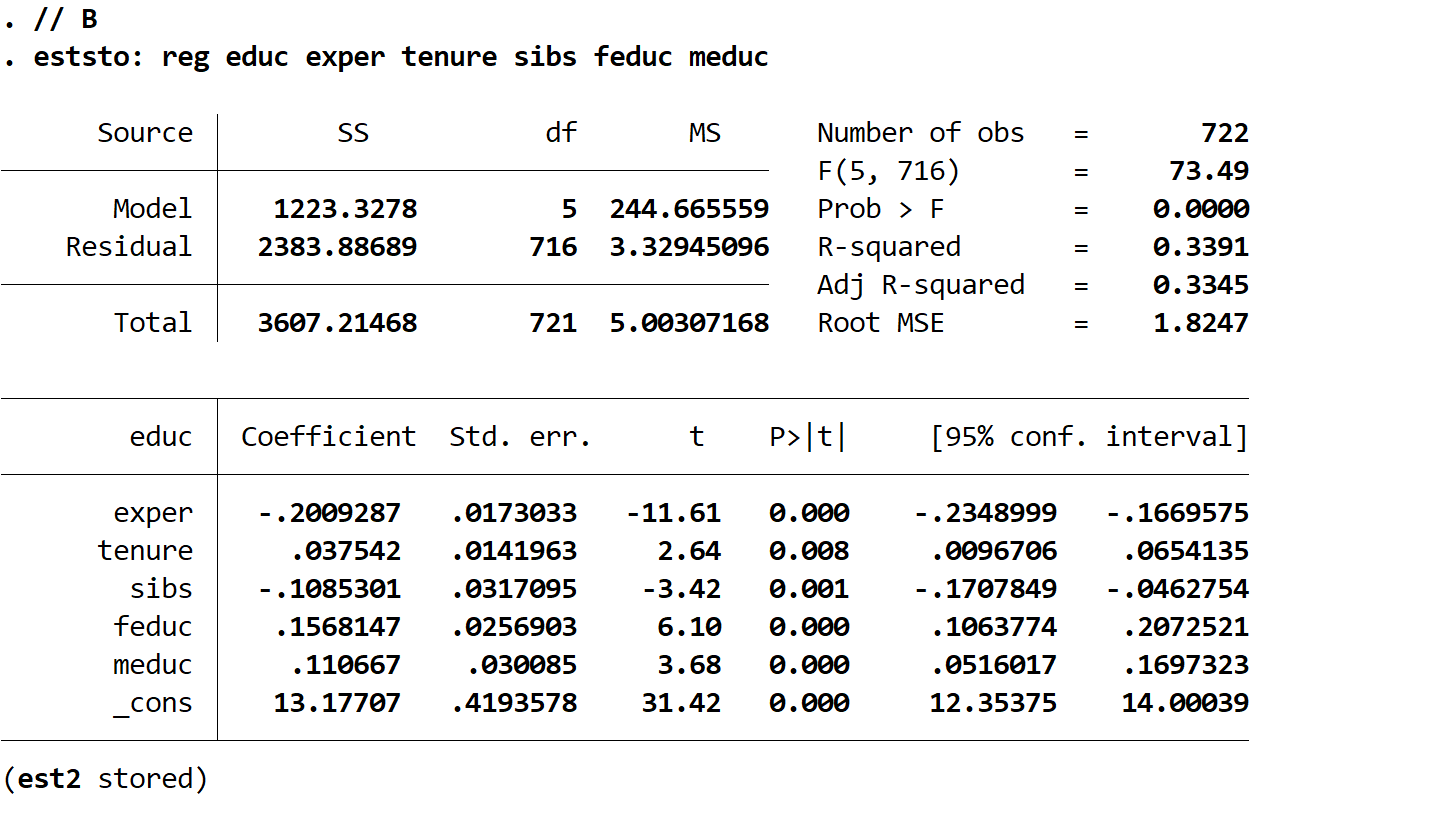
\includegraphics[width=0.8\textwidth]{Figure/P3.2.jpg}  

    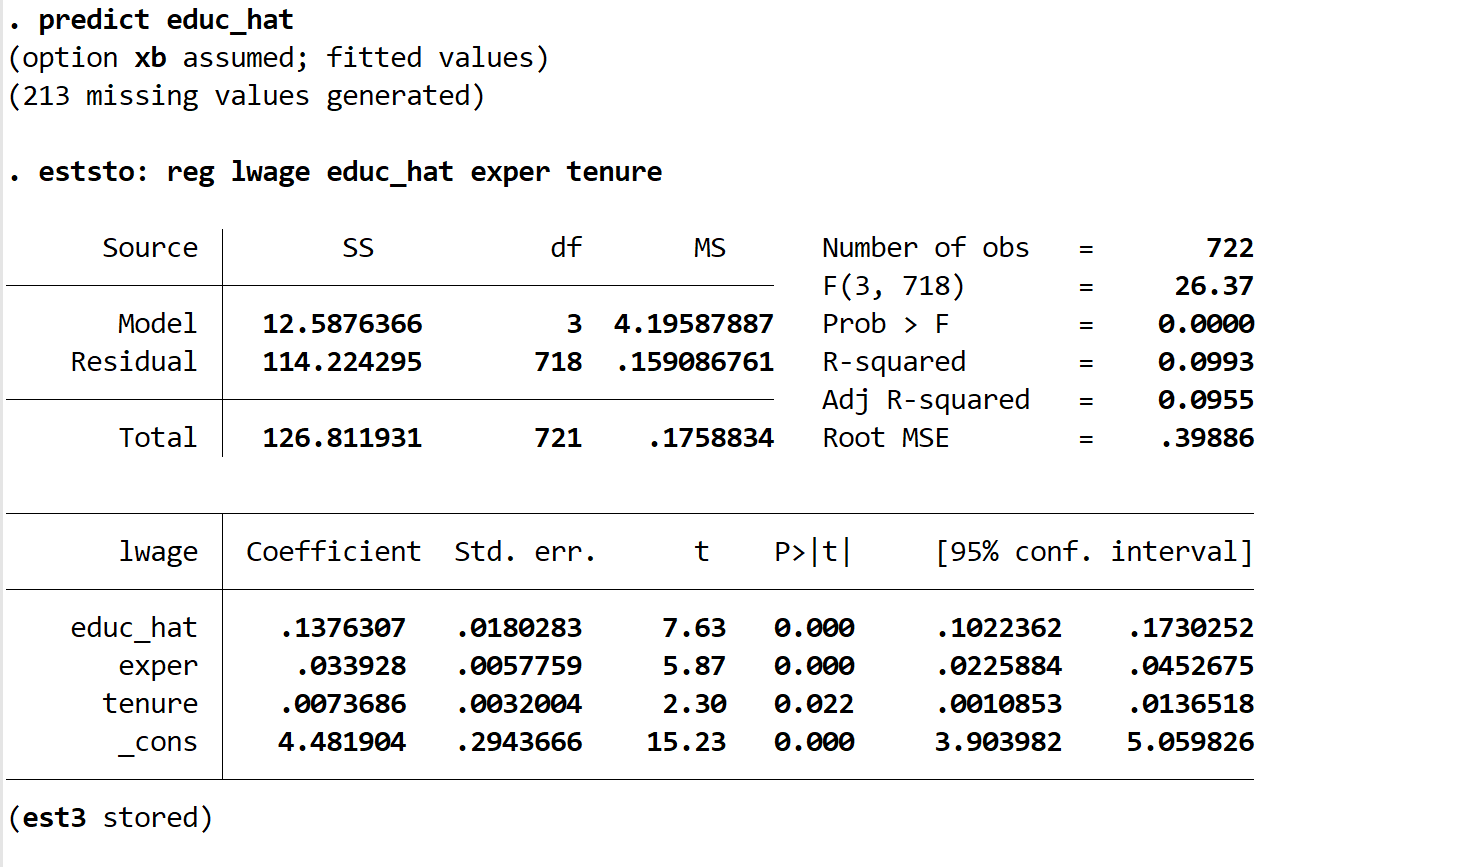
\includegraphics[width=0.8\textwidth]{Figure/P3.3.jpg}

    \includegraphics[width=0.8\textwidth]{Figure/P3.4.jpg}
\end{center}

We can notice that all estimates $\beta_j$ are identical to those obtained before, but that the standard errors in the second equation are different. In the second case, the estimate of $\sigma^2$ is wrong. Its computation includes the variance of the sum of the error term in the second equation and the error term from the first stage regression. Since $\hat{X}$ is a projection of $X$, 2SLS will have higher variance (even if OLS is inconsistent). This confirms the fact that, when OLS is consistent, it is better than 2SLS. But when $X$ is endogenous, we must account for endogeneity using the 2SLS procedure. In summary, we can conclude that standard errors from the second approach are invalid.

\begin{center}


    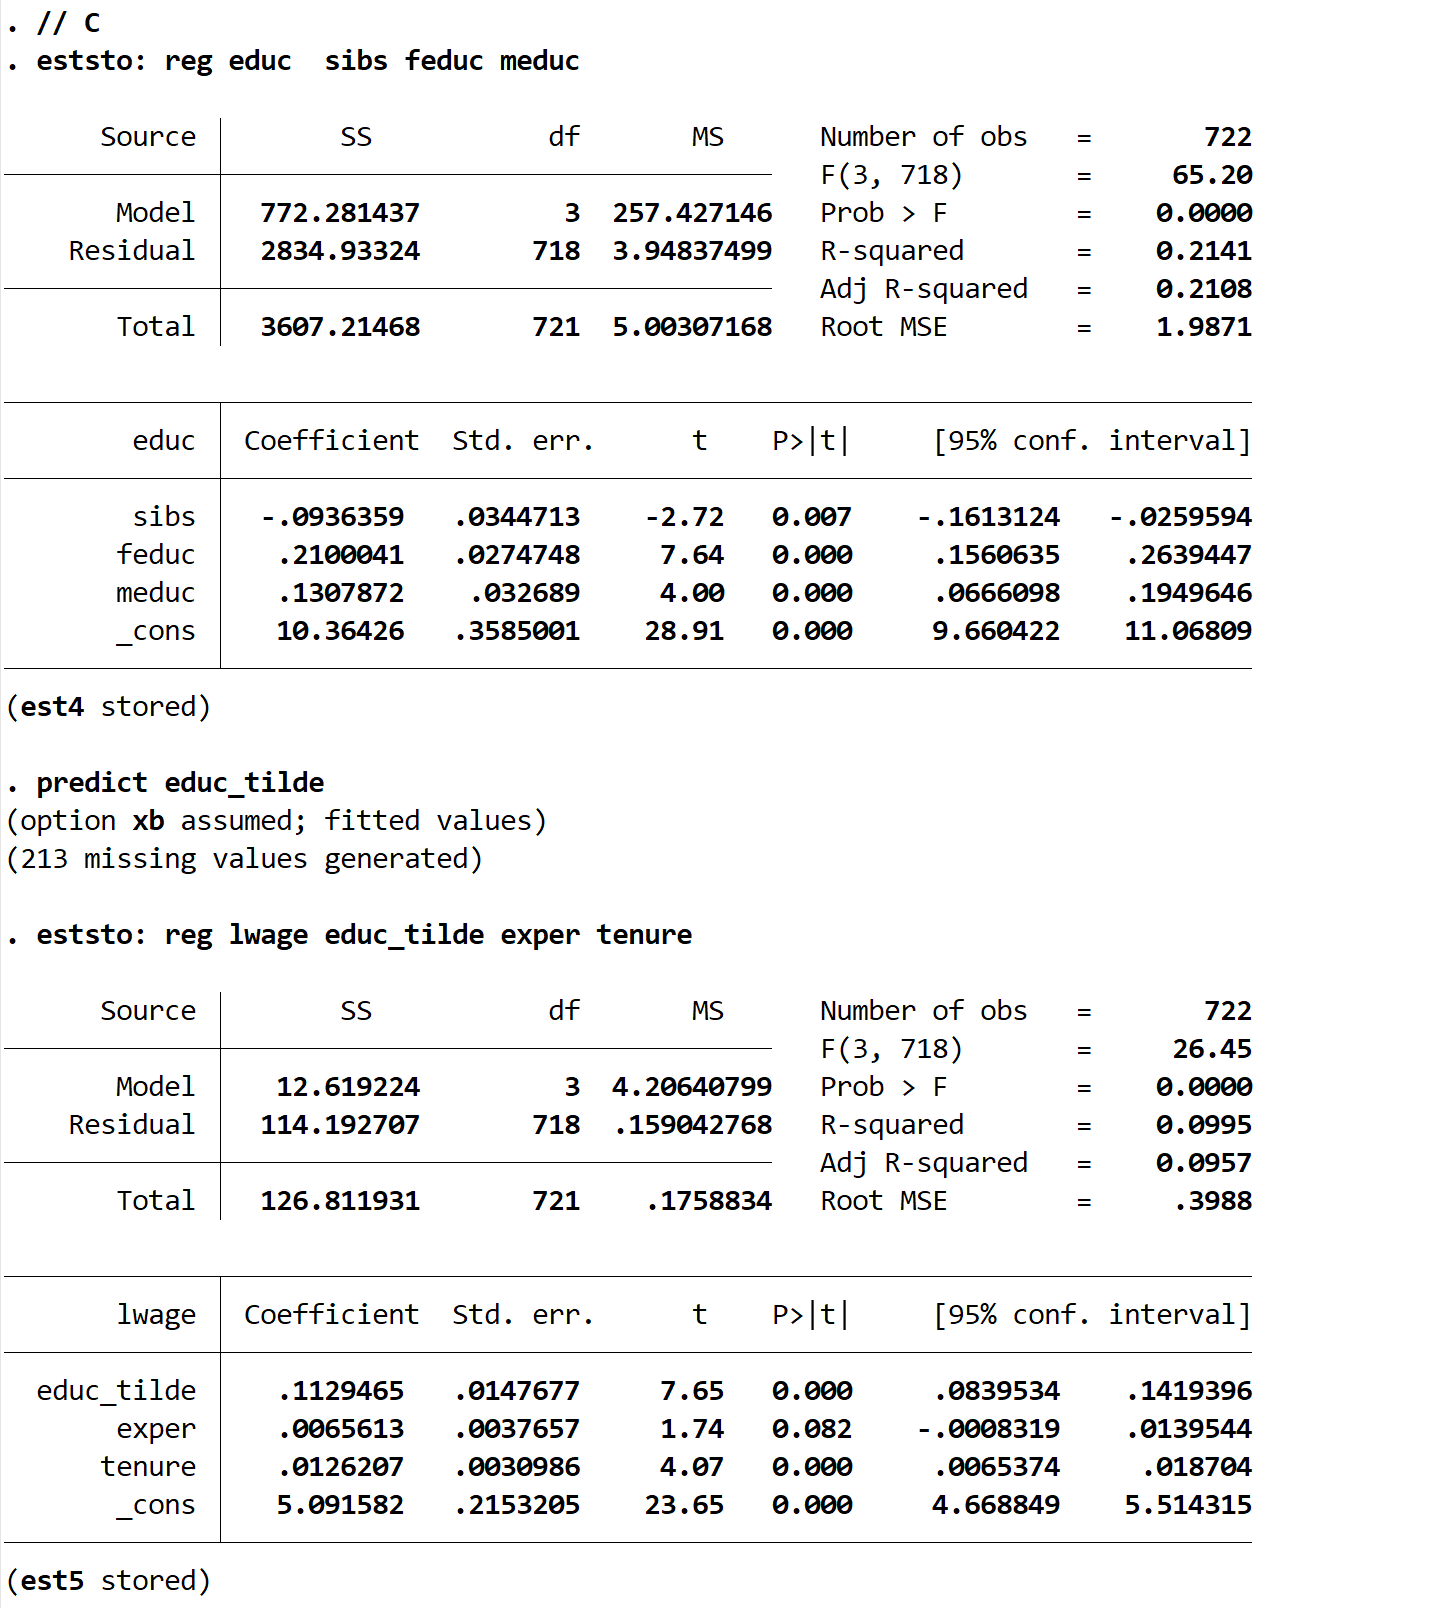
\includegraphics[width=0.8\textwidth]{Figure/P3.5.jpg}

    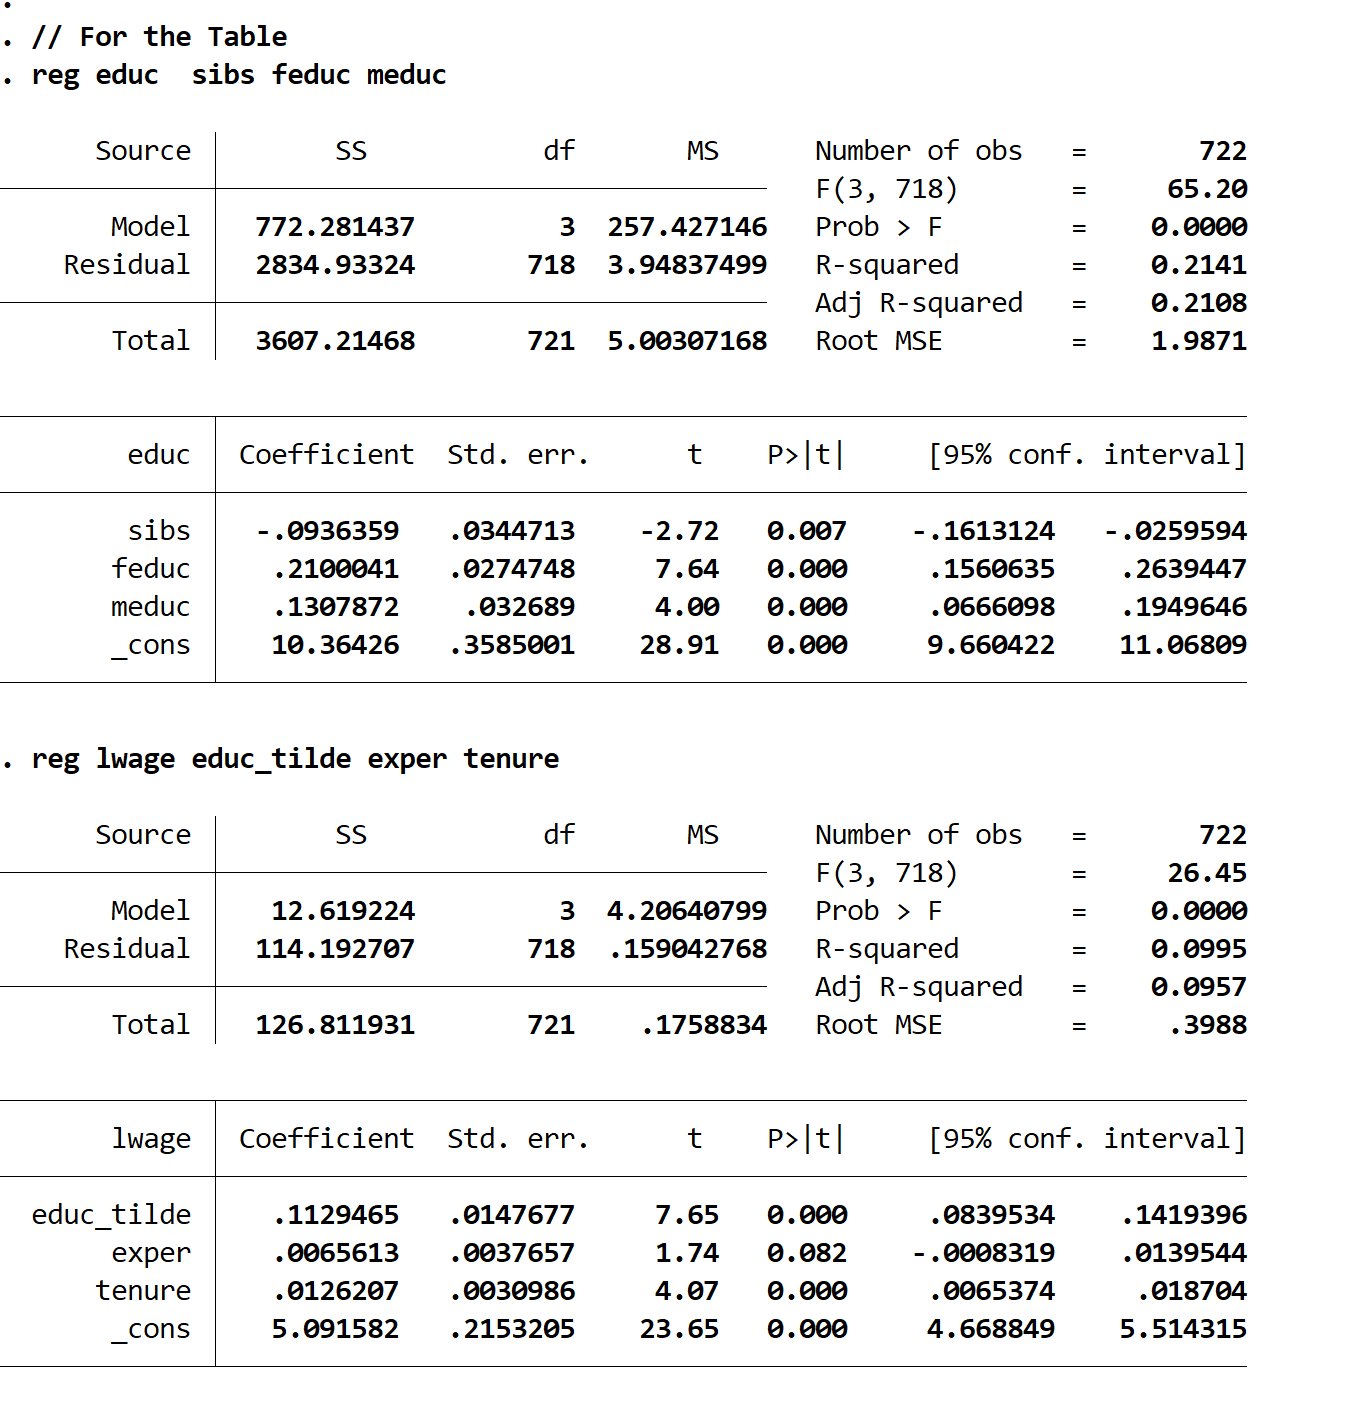
\includegraphics[width=0.8\textwidth]{Figure/P3.6.jpg}
\end{center}

The first stage is used to estimate the endogenous variable, and if the first stage is not correctly specified, the second stage will not be consistent. The error term in the second stage will not be orthogonal to the exogenous regressors and the estimator will be inconsistent. 

\begin{center}

    \includegraphics[width=0.8\textwidth]{Figure/P3.7.jpg}

    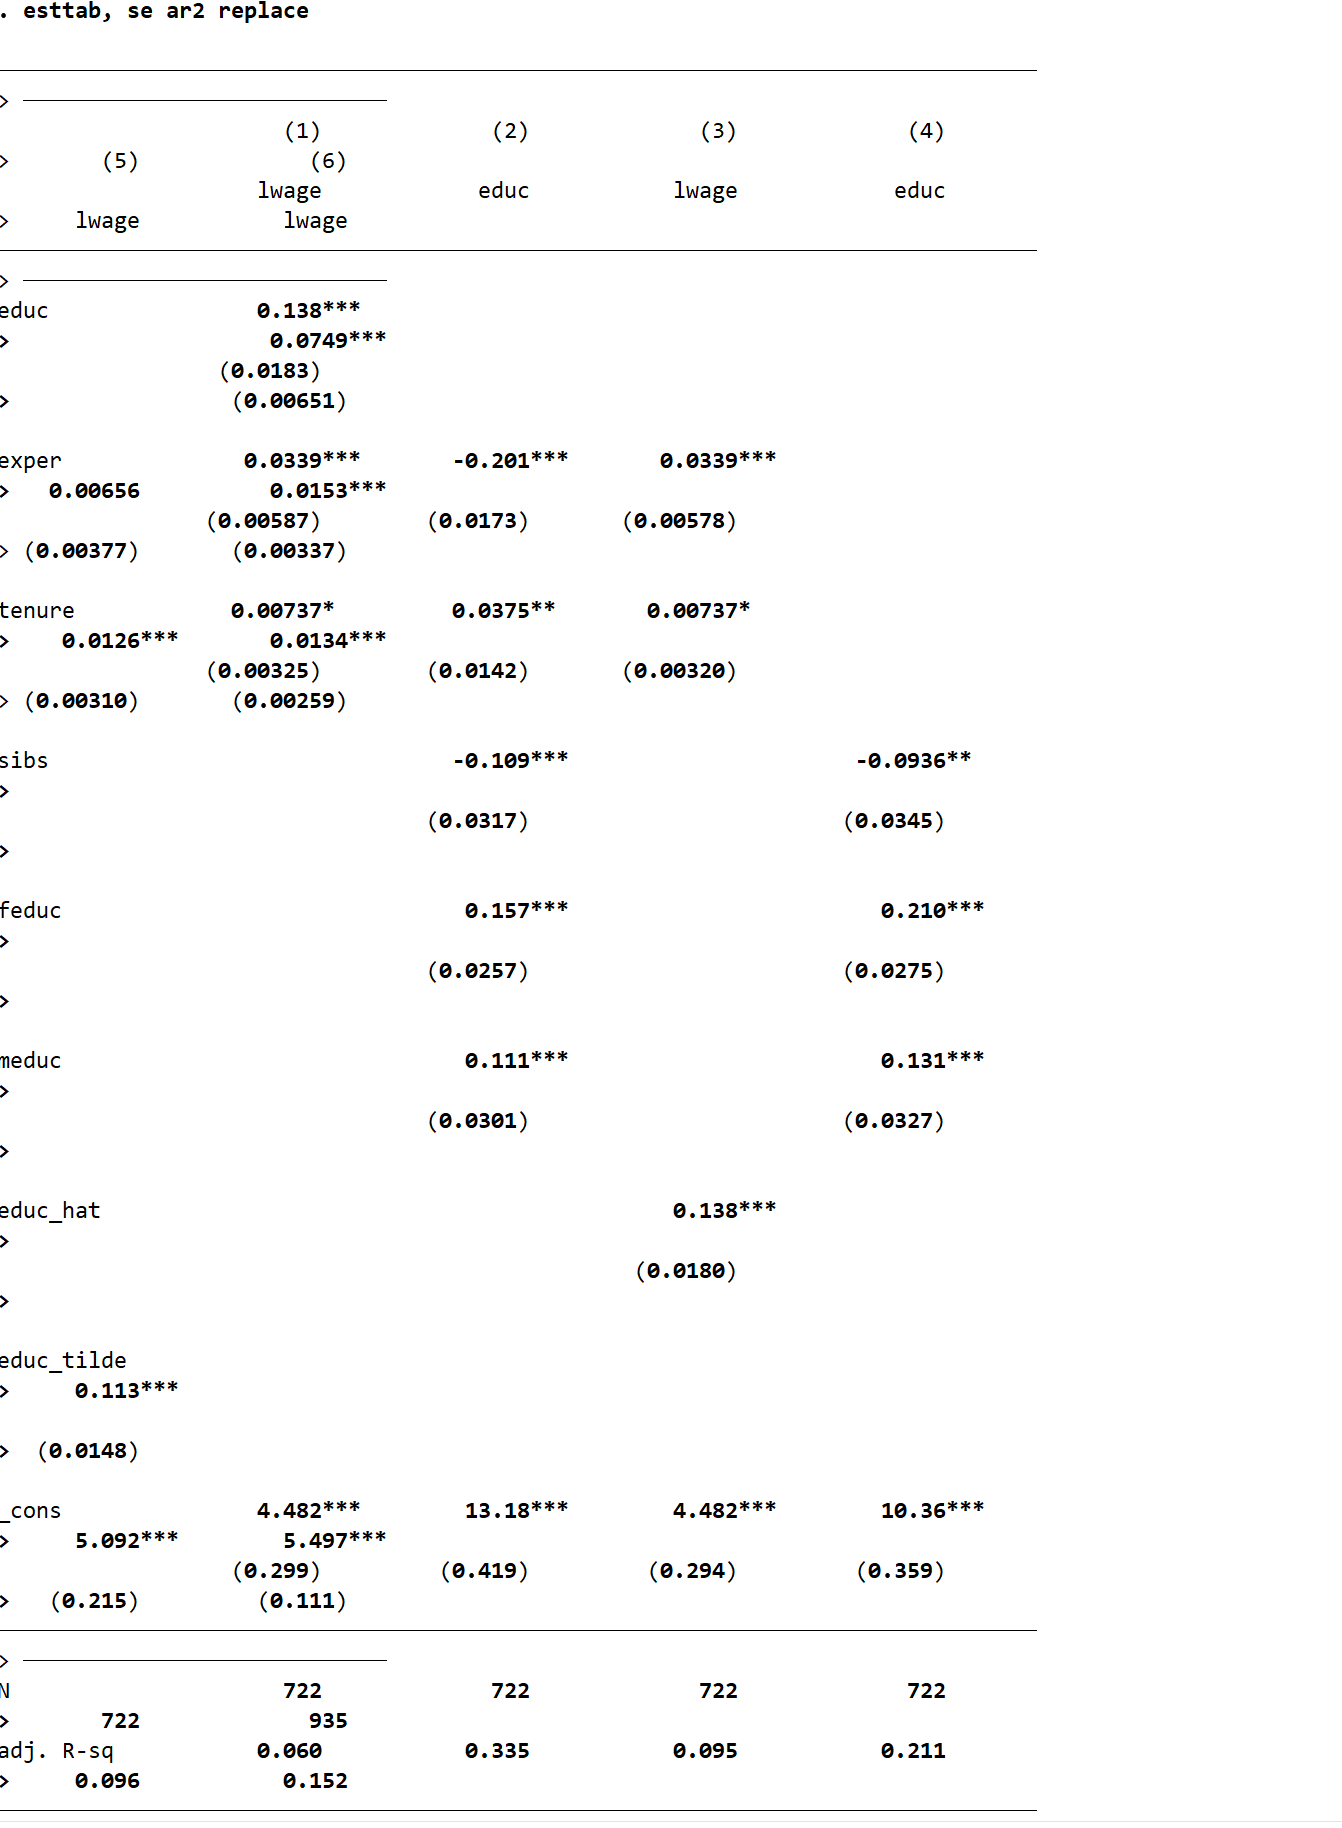
\includegraphics[width=0.8\textwidth]{Figure/P3.8.jpg}

\end{center}

\section{Question 4}
\textbf{Solution:}

\begin{center}
    
    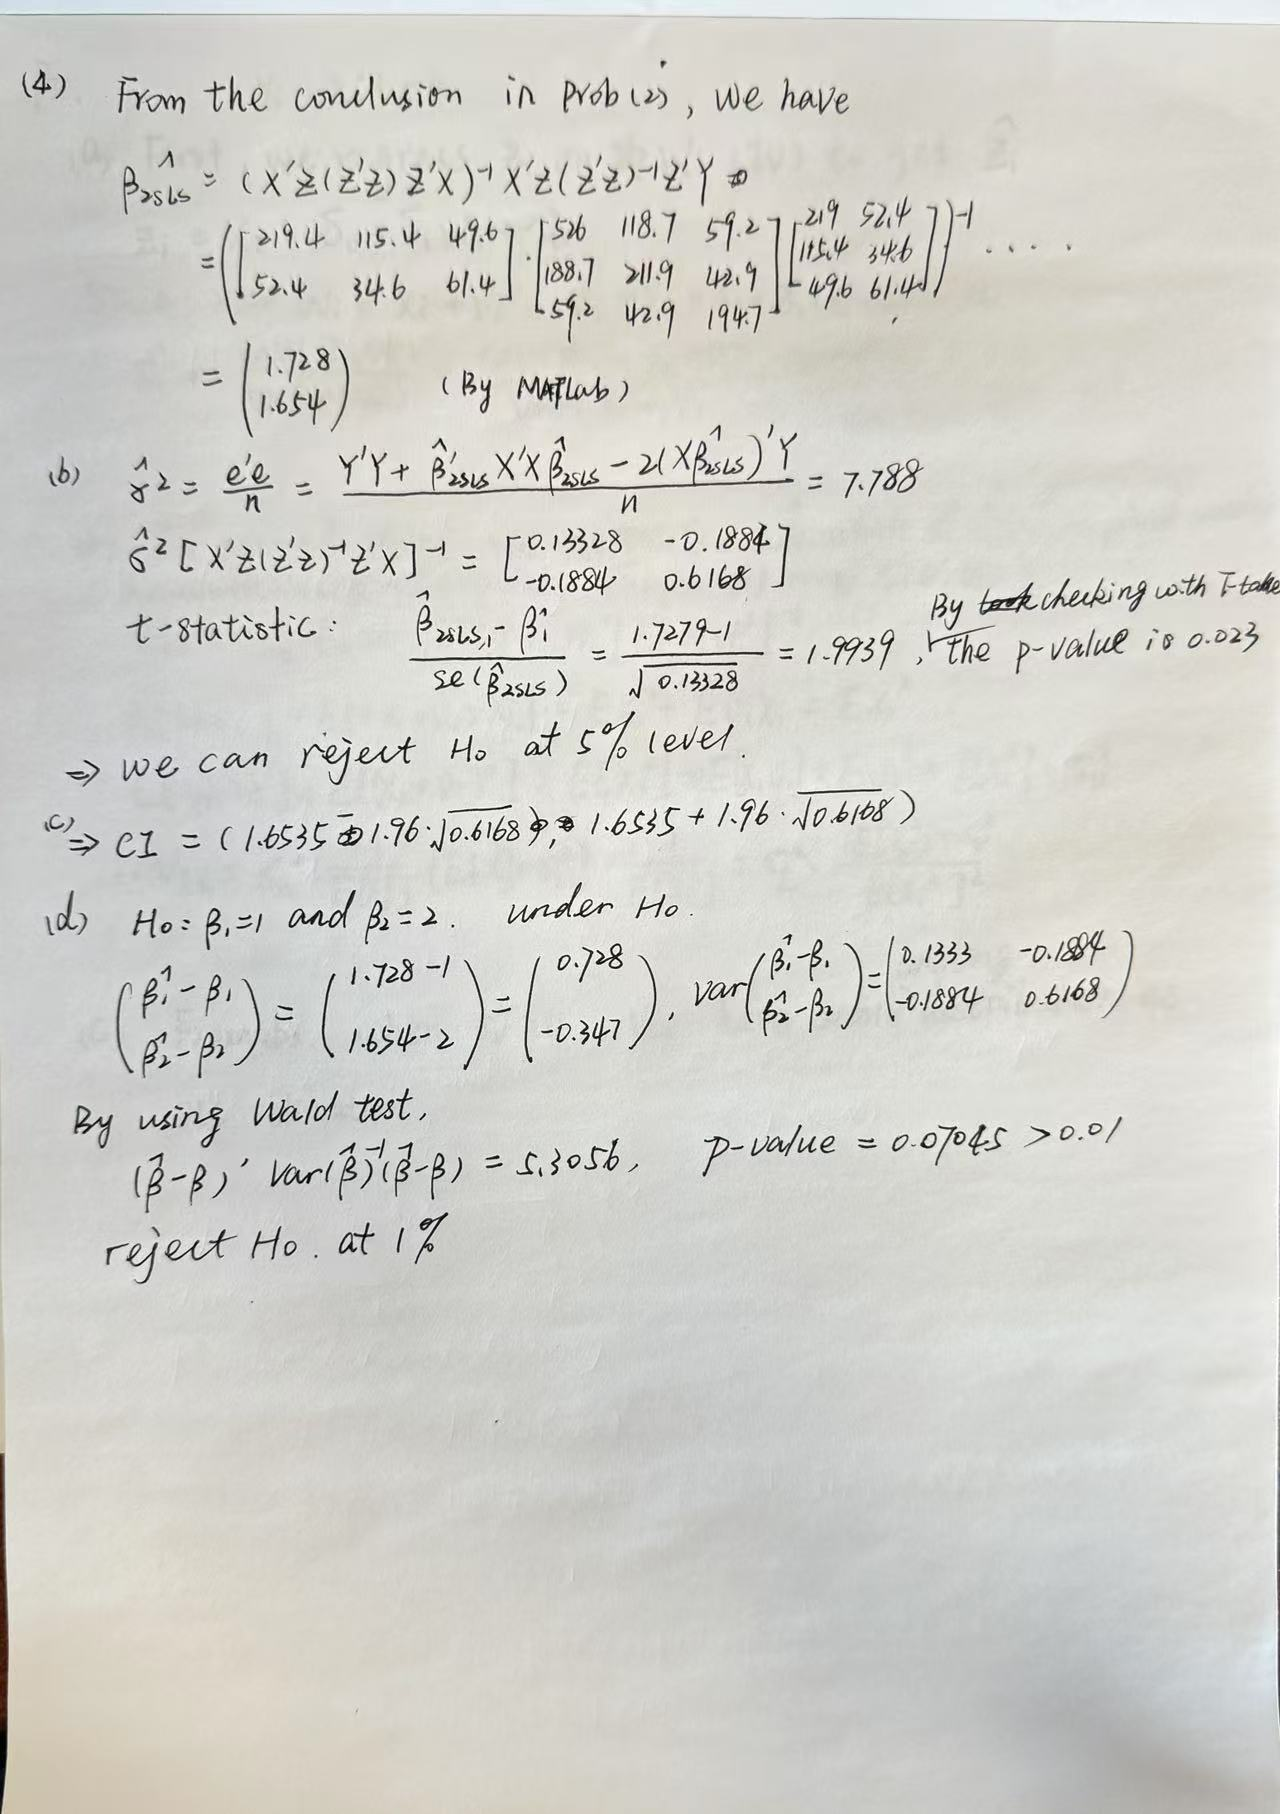
\includegraphics[width=0.8\textwidth]{Figure/P4.jpg}

\end{center}
\section{Question 5}
\textbf{Solution:}

\begin{center}
    
    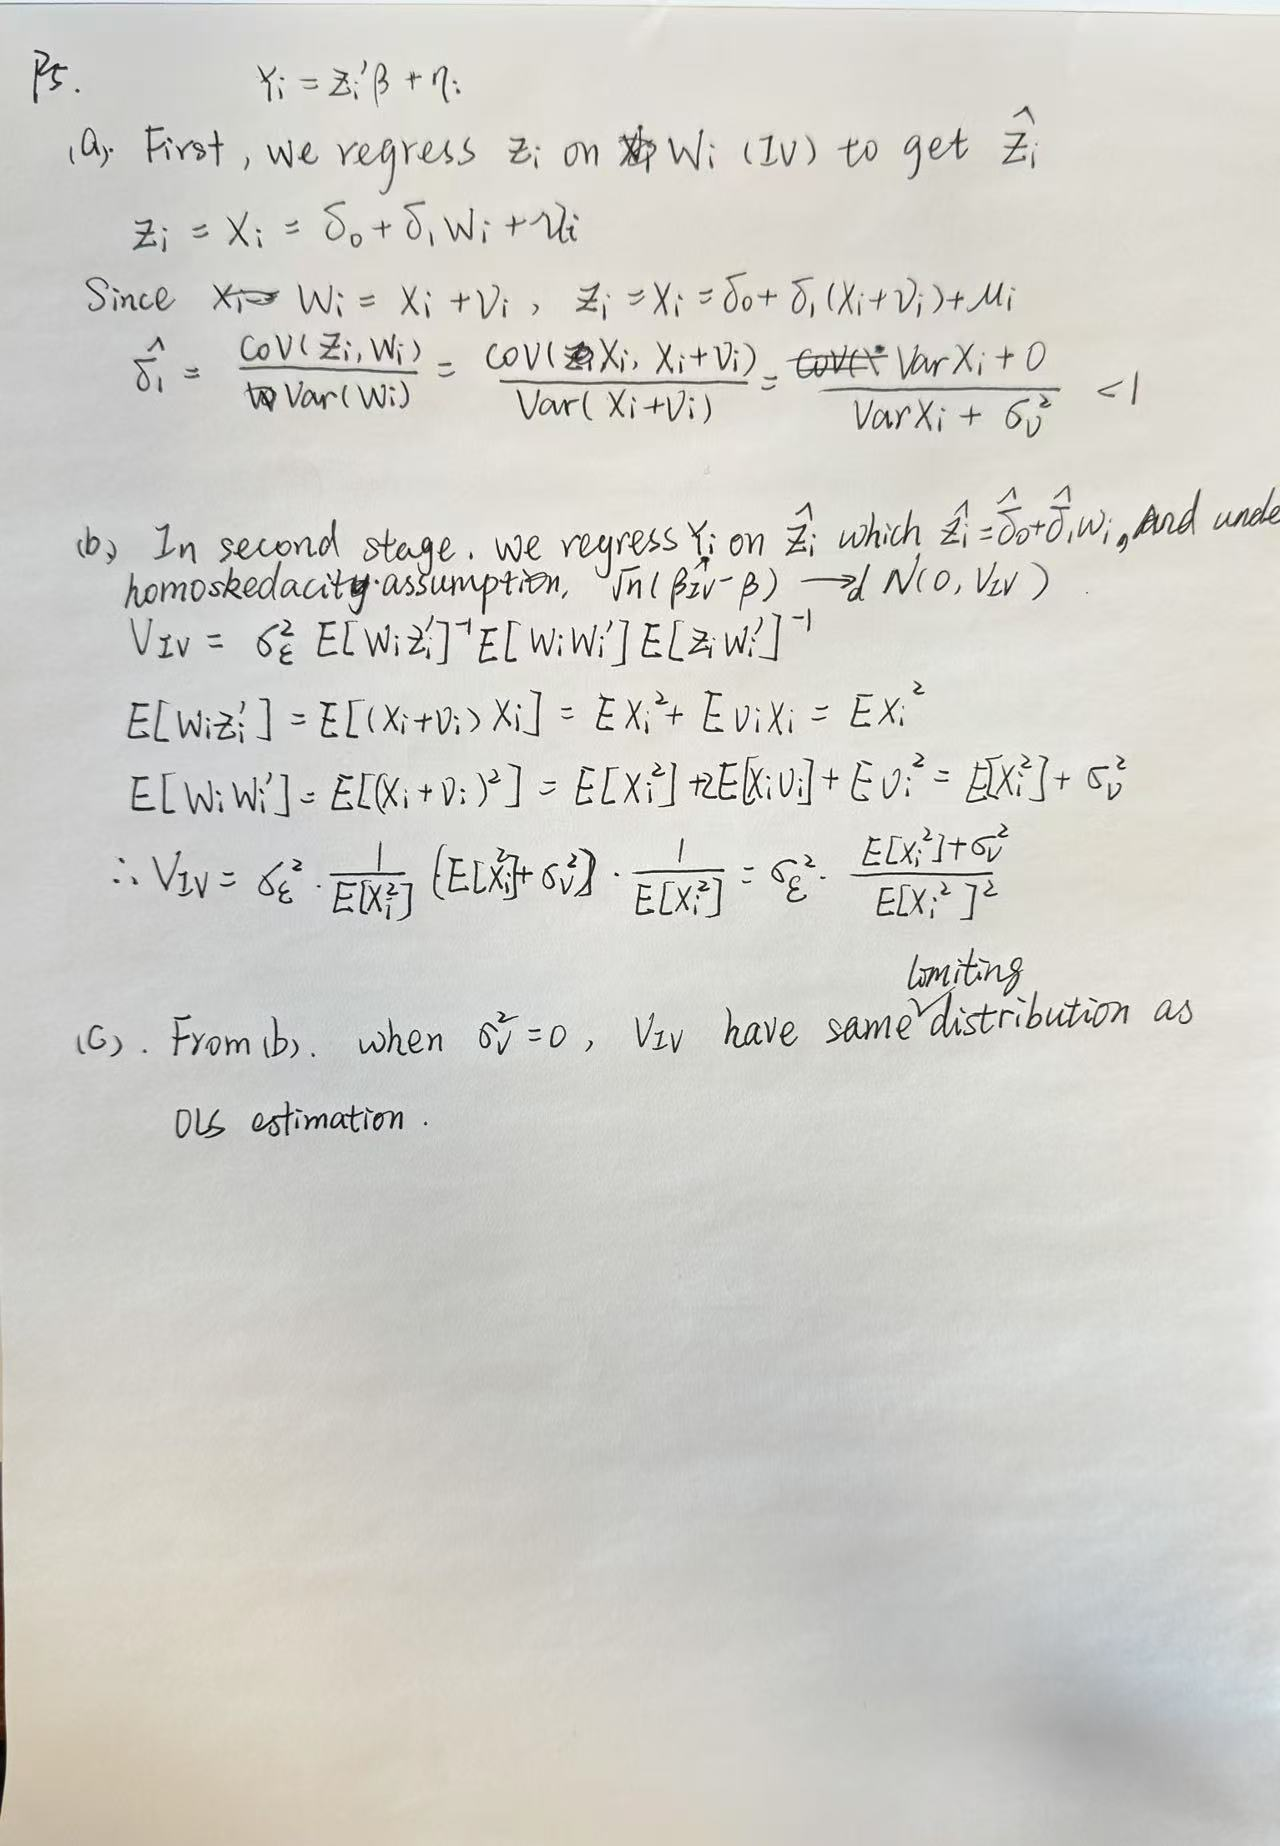
\includegraphics[width=0.8\textwidth]{Figure/P5.jpg}
\end{center}

\end{document}